%
%  This is an example of how a LaTeX thesis should be formatted.  This
%  document contains chapter 2 of the thesis.
%
%  Time-stamp: "[sample-chapter2.tex] last modified by Scott Budge (scott) on 2016-07-28 (Thursday, 28 July 2016) at 08:40:50 on goga.ece.usu.edu"
%
%  Info: $Id: sample-chapter2.tex 967 2016-07-28 15:33:29Z scott $   USU
%  Revision: $Rev: 967 $
% $LastChangedDate: 2016-07-28 09:33:29 -0600 (Thu, 28 Jul 2016) $
% $LastChangedBy: scott $
%

\chapter{Research and Design Methods}

This chapter describes the design and implementation of the active snore cancellation system. First, the fractional delay interpolation method used for microphone array alignment is presented. Next, the mechanical platform and supporting electronics are described. Finally, the adaptive filtering algorithms used for active noise cancellation are introduced, culminating in the Fast Array Recursive Least Squares (FARLS) algorithm employed throughout this work.

\section{Array Processing Using Sinc Interpolation}

To enable accurate time alignment across the microphone array, a fractional delay filtering approach based on sinc interpolation was selected. Sinc interpolation is well-suited for broadband signals, as it provides exact reconstruction for bandlimited signals according to the Shannon-Whittaker sampling theorem. Since snore signals exhibit broadband characteristics, this approach preserves signal fidelity during delay compensation.

A continuous-time delayed signal can be expressed using the Shannon-Whittaker interpolation formula as

\begin{equation}
s(t - \tau) = \sum_{l=-\infty}^{\infty} s(lT) \, \text{sinc}\left(2B(t - \tau - lT)\right),
\end{equation}

where $T$ is the sampling period, $B$ is the signal bandwidth, and $\tau$ is the desired delay.

In practice, the infinite summation is not realizable. Therefore, the interpolation is approximated by truncating the sinc function to a finite number of terms:

\begin{equation}
s(t - \tau) = \sum_{l=-P}^{P} s(lT) \, \text{sinc}\left(2B(t - \tau - lT)\right),
\end{equation}

where $P$ determines the length of the interpolation filter.

Sampling the delayed signal at discrete time instances $t = nT$ yields

\begin{equation}
s(nT - \tau) = \sum_{l=-P}^{P} s(lT) \, \text{sinc}\left(2B(nT - lT - \tau)\right).
\end{equation}

This expression can be interpreted as a finite impulse response (FIR) filter that implements both integer and fractional delay. The integer (bulk) delay accounts for whole sample shifts, while the fractional delay is achieved through sinc-based interpolation.

A real-time implementation of this approach was developed in C. For each sensor in the array, the required delay was decomposed into an integer delay component and a fractional delay component. The integer delay was implemented using a buffer offset, while the fractional delay was realized using the truncated sinc interpolation filter.

To compute the required delay at each microphone, the propagation delay from the acoustic source to each sensor was first estimated. Let the maximum delay across all microphones be denoted as $\tau_{\text{max}}$. The relative delay applied to the $i$-th microphone is then computed as

\begin{equation}
\tau_i = \tau_{\text{max}} - \tau_{\text{mic},i},
\end{equation}

where $\tau_{\text{mic},i}$ is the propagation delay from the source to the $i$-th microphone. This relative delay ensures that signals from all microphones are temporally aligned, effectively compensating for differences in propagation time. As a result, the array achieves constructive combination of the received signals, producing the desired array gain.

The interpolation length $P$ determines the trade-off between computational complexity and interpolation accuracy. In this work, a value of $P = 10$ was selected, resulting in a filter length of $2P + 1$. This value was chosen empirically, as it provided sufficient interpolation accuracy while maintaining computational efficiency for real-time implementation.

This approach enables precise time alignment across the microphone array, which is critical for accurate near-field localization and subsequent adaptive noise control processing.

\section{Mechanical Layout}

The microphone array developed during previous work provided only a rudimentary test platform with limited ability to adjust microphone spacing and sensor height. To improve experimental flexibility, a new adjustable test structure was designed and constructed.

\begin{figure}[H]
    \centering
    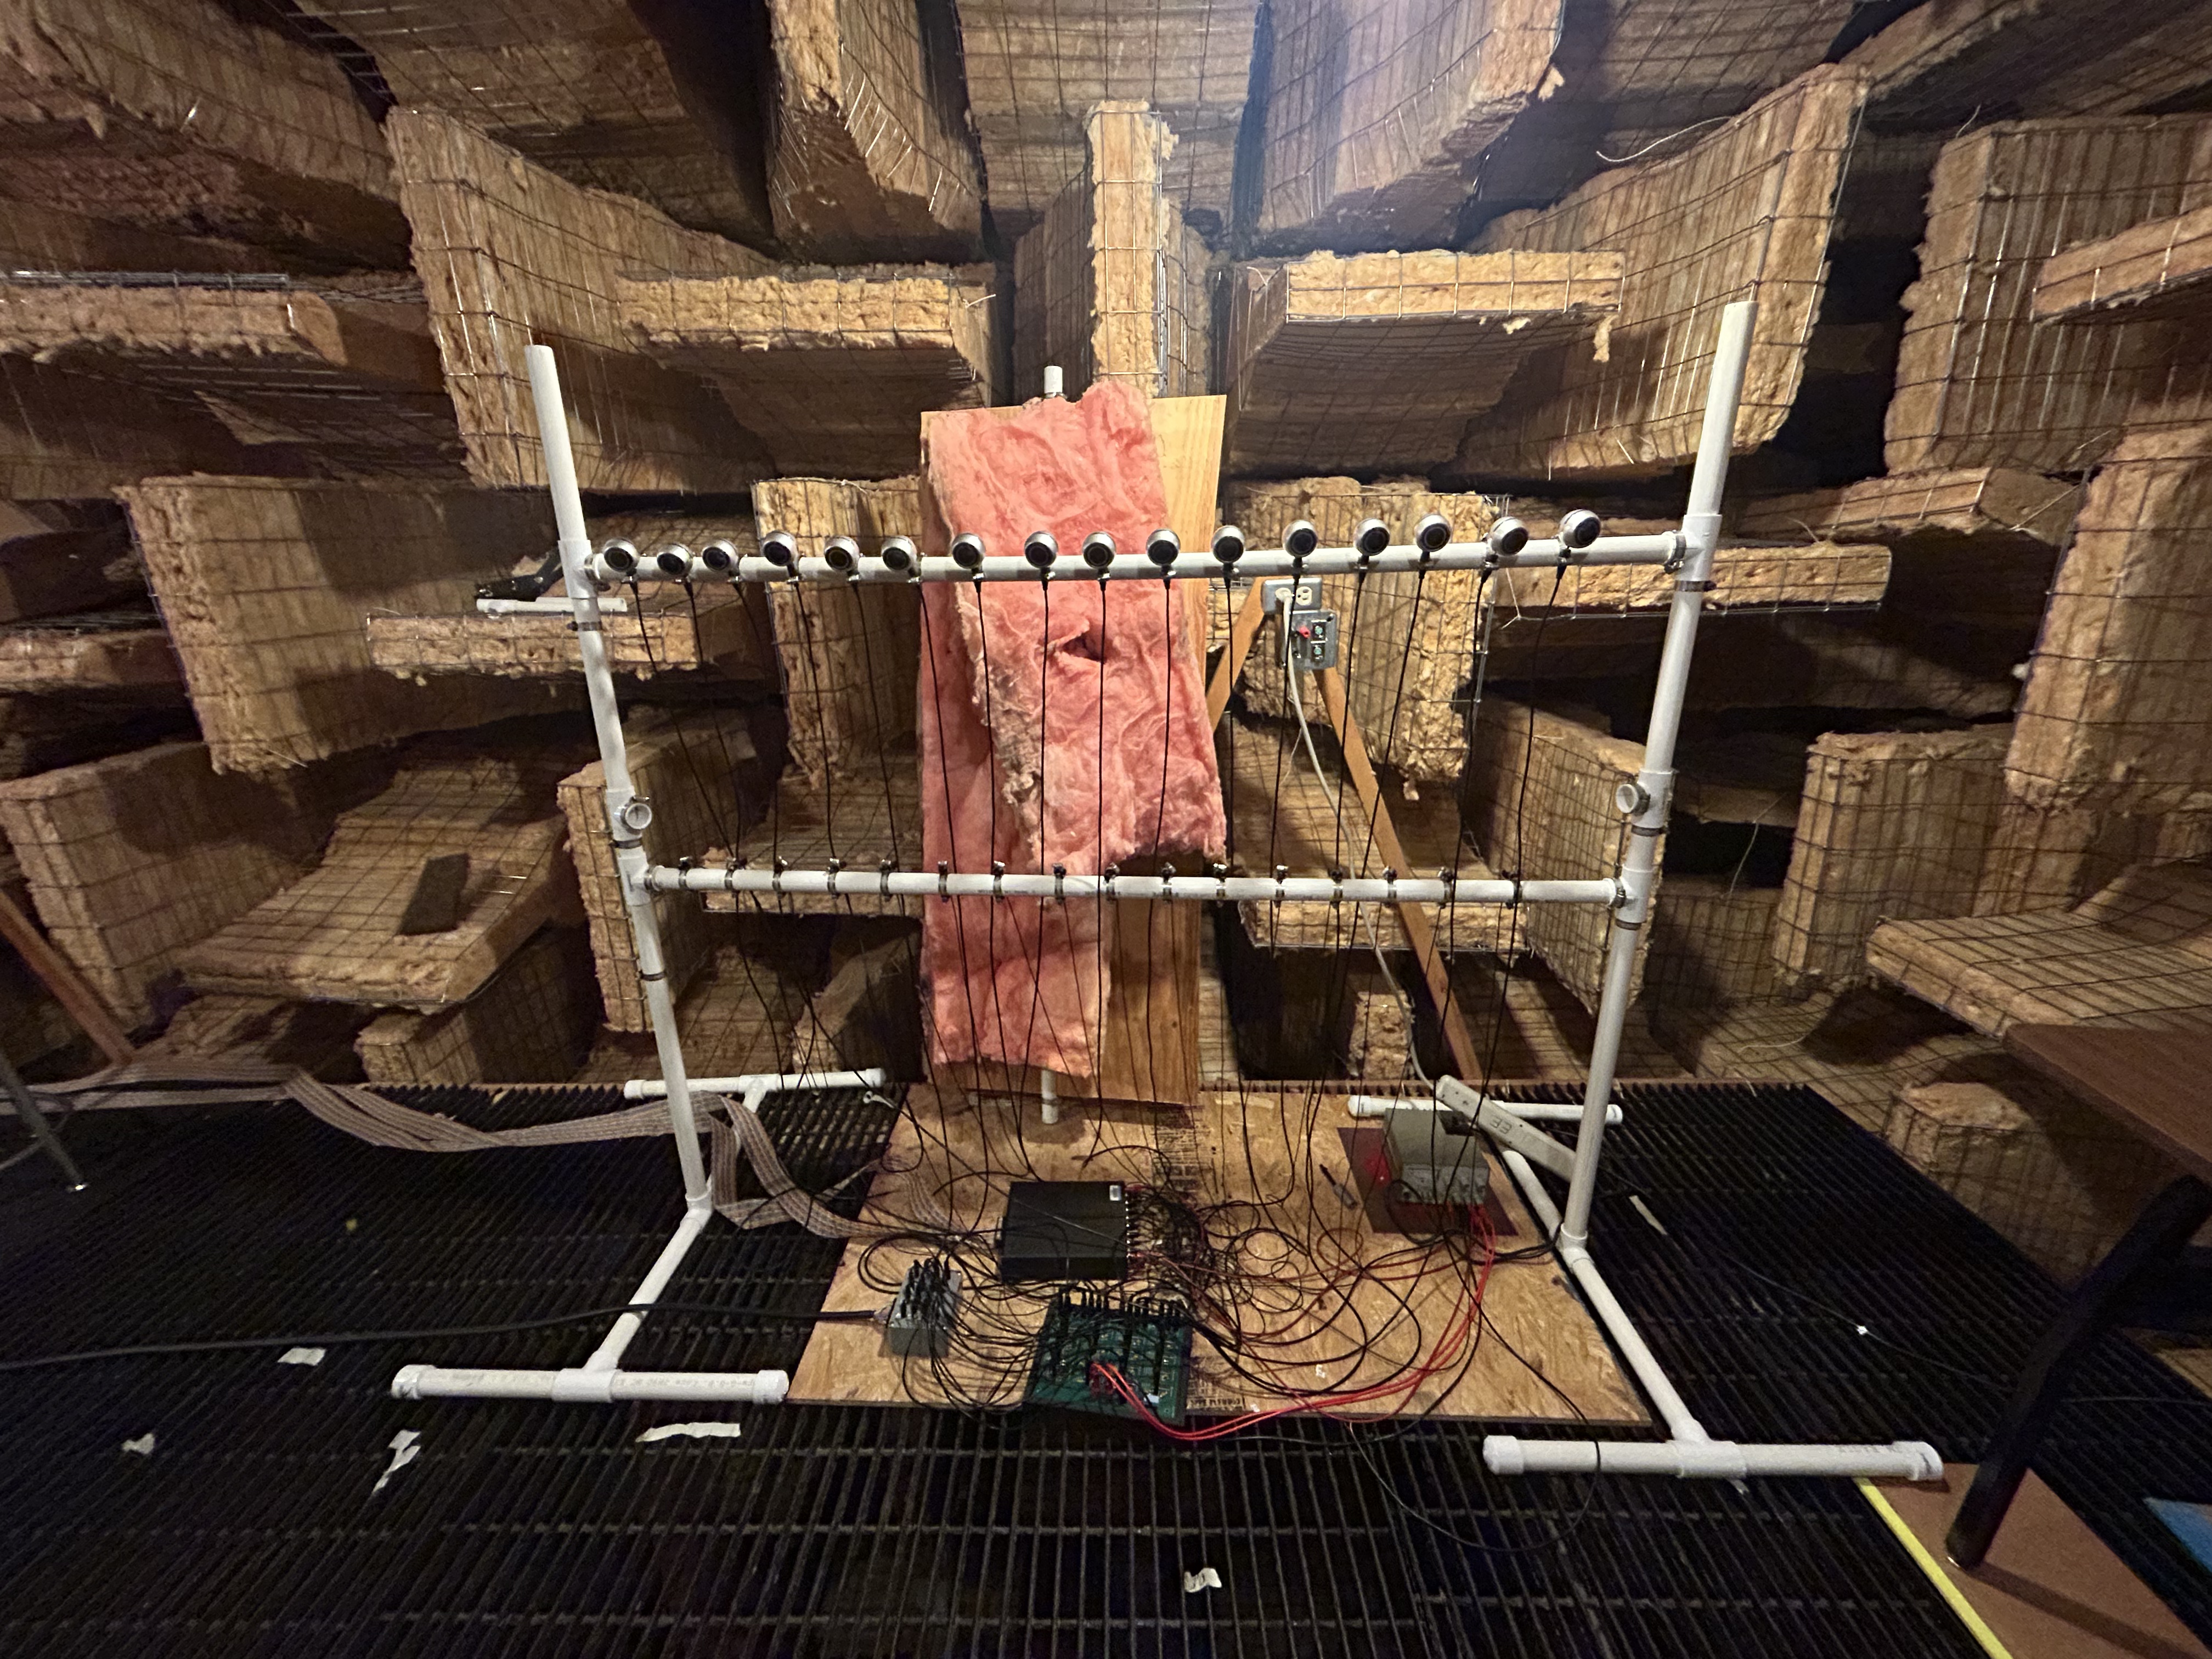
\includegraphics[width=0.8\textwidth]{array_hardware.png}
    \caption{Adjustable mechanical structure constructed for the microphone and speaker array, providing configurable sensor spacing and height.}
    \label{fig:Array_setup}
\end{figure}

The support structure was built using PVC pipe and standard PVC fittings to provide a lightweight, low-cost, and easily reconfigurable platform. The design allows the height of the microphone array, the spacing between individual microphones, and the orientation of the array to be adjusted. These adjustable parameters enable the array geometry to be modified for different experimental configurations and localization scenarios.

To facilitate complete system testing, a loudspeaker array was incorporated into the same support structure. The loudspeaker array was designed independently of the microphone array, allowing its height, orientation, and position to be adjusted without affecting the microphone geometry. This arrangement provides a repeatable experimental setup for evaluating signal acquisition, beamforming, and adaptive noise control algorithms.

To reduce acoustic crosstalk between the loudspeaker array and the microphone array during testing, a removable sound baffle was constructed. The baffle consisted of a PVC frame with a plywood panel covered in acoustic insulation. The design allowed the baffle to be repositioned and adjusted in both height and orientation, providing flexibility for different experimental configurations while reducing direct acoustic coupling between the arrays.

\begin{figure}[H]
    \centering
    \includegraphics[width=0.48\textwidth]{Data/Photos/Ribbon_cable_box.png}
    \caption{Custom interface enclosure used to provide connections between the microphone array and the linux machine.}
    \label{fig:Ribbon_box}
\end{figure}


A custom interface enclosure was also designed to connect the loudspeaker array to the digital-to-analog converter (DAC) installed in the host computer. The enclosure accepts the ribbon cable output from the DAC and routes each channel to standard 3.5 mm audio connectors. The enclosure was fabricated from a plastic box using a manual milling machine to create the required openings for the connectors. Internal wiring was completed by soldering each ribbon cable conductor to its corresponding 3.5 mm audio jack.

Initial testing indicated that the DAC output contained significant high-frequency components associated with the stepped output waveform, producing audible distortion in the loudspeakers. To reduce these artifacts, an analog low-pass filter bank was designed and incorporated between the DAC outputs and the speakers. Unlike the interface enclosure, the filter enclosure was manufactured using additive manufacturing (3D printing). The enclosure was designed in Onshape using the PCB model, allowing a custom enclosure to be produced that accurately supported the assembled circuit board while simplifying fabrication.

The completed mechanical and electrical test platform provides a configurable environment for evaluating microphone array processing, loudspeaker placement, and future adaptive noise control experiments.

\section{Additional Electronics}

As described in the previous section, a custom interface enclosure was constructed to connect the ribbon cable output of the digital-to-analog converter (DAC) to standard 3.5 mm audio connectors. This required soldering each conductor of the ribbon cable connector to its corresponding 3.5 mm audio jack, providing a reliable electrical interface between the DAC and the loudspeaker array.

The DAC reproduces digital signals using a zero-order hold, resulting in a stepped output waveform. Although the desired audio signal lies within the audible frequency range, the stepped waveform also contains unwanted high-frequency spectral components. Because the loudspeakers are capable of reproducing frequencies across much of the audible spectrum, these high-frequency components introduced audible distortion during testing.

To reduce these artifacts, a programmable analog low-pass filter bank was designed and constructed. Since multiple sampling frequencies were anticipated during experimentation, a fixed cutoff frequency was not suitable. Instead, a programmable filter architecture was selected, allowing the cutoff frequency to be adjusted as needed for different sampling rates while maintaining adequate suppression of the high-frequency DAC images.

The filter bank was implemented using the MAX270CPP+ programmable analog filter integrated circuit. A custom printed circuit board (PCB) was designed and manufactured to interface with the device. The PCB accepts standard 3.5 mm audio inputs from the DAC interface enclosure and provides filtered 3.5 mm outputs for connection to the loudspeaker array. The programmable filter integrated circuits were configured through software, allowing the filter characteristics to be modified without redesigning the hardware.

\begin{figure}[H]
    \centering
    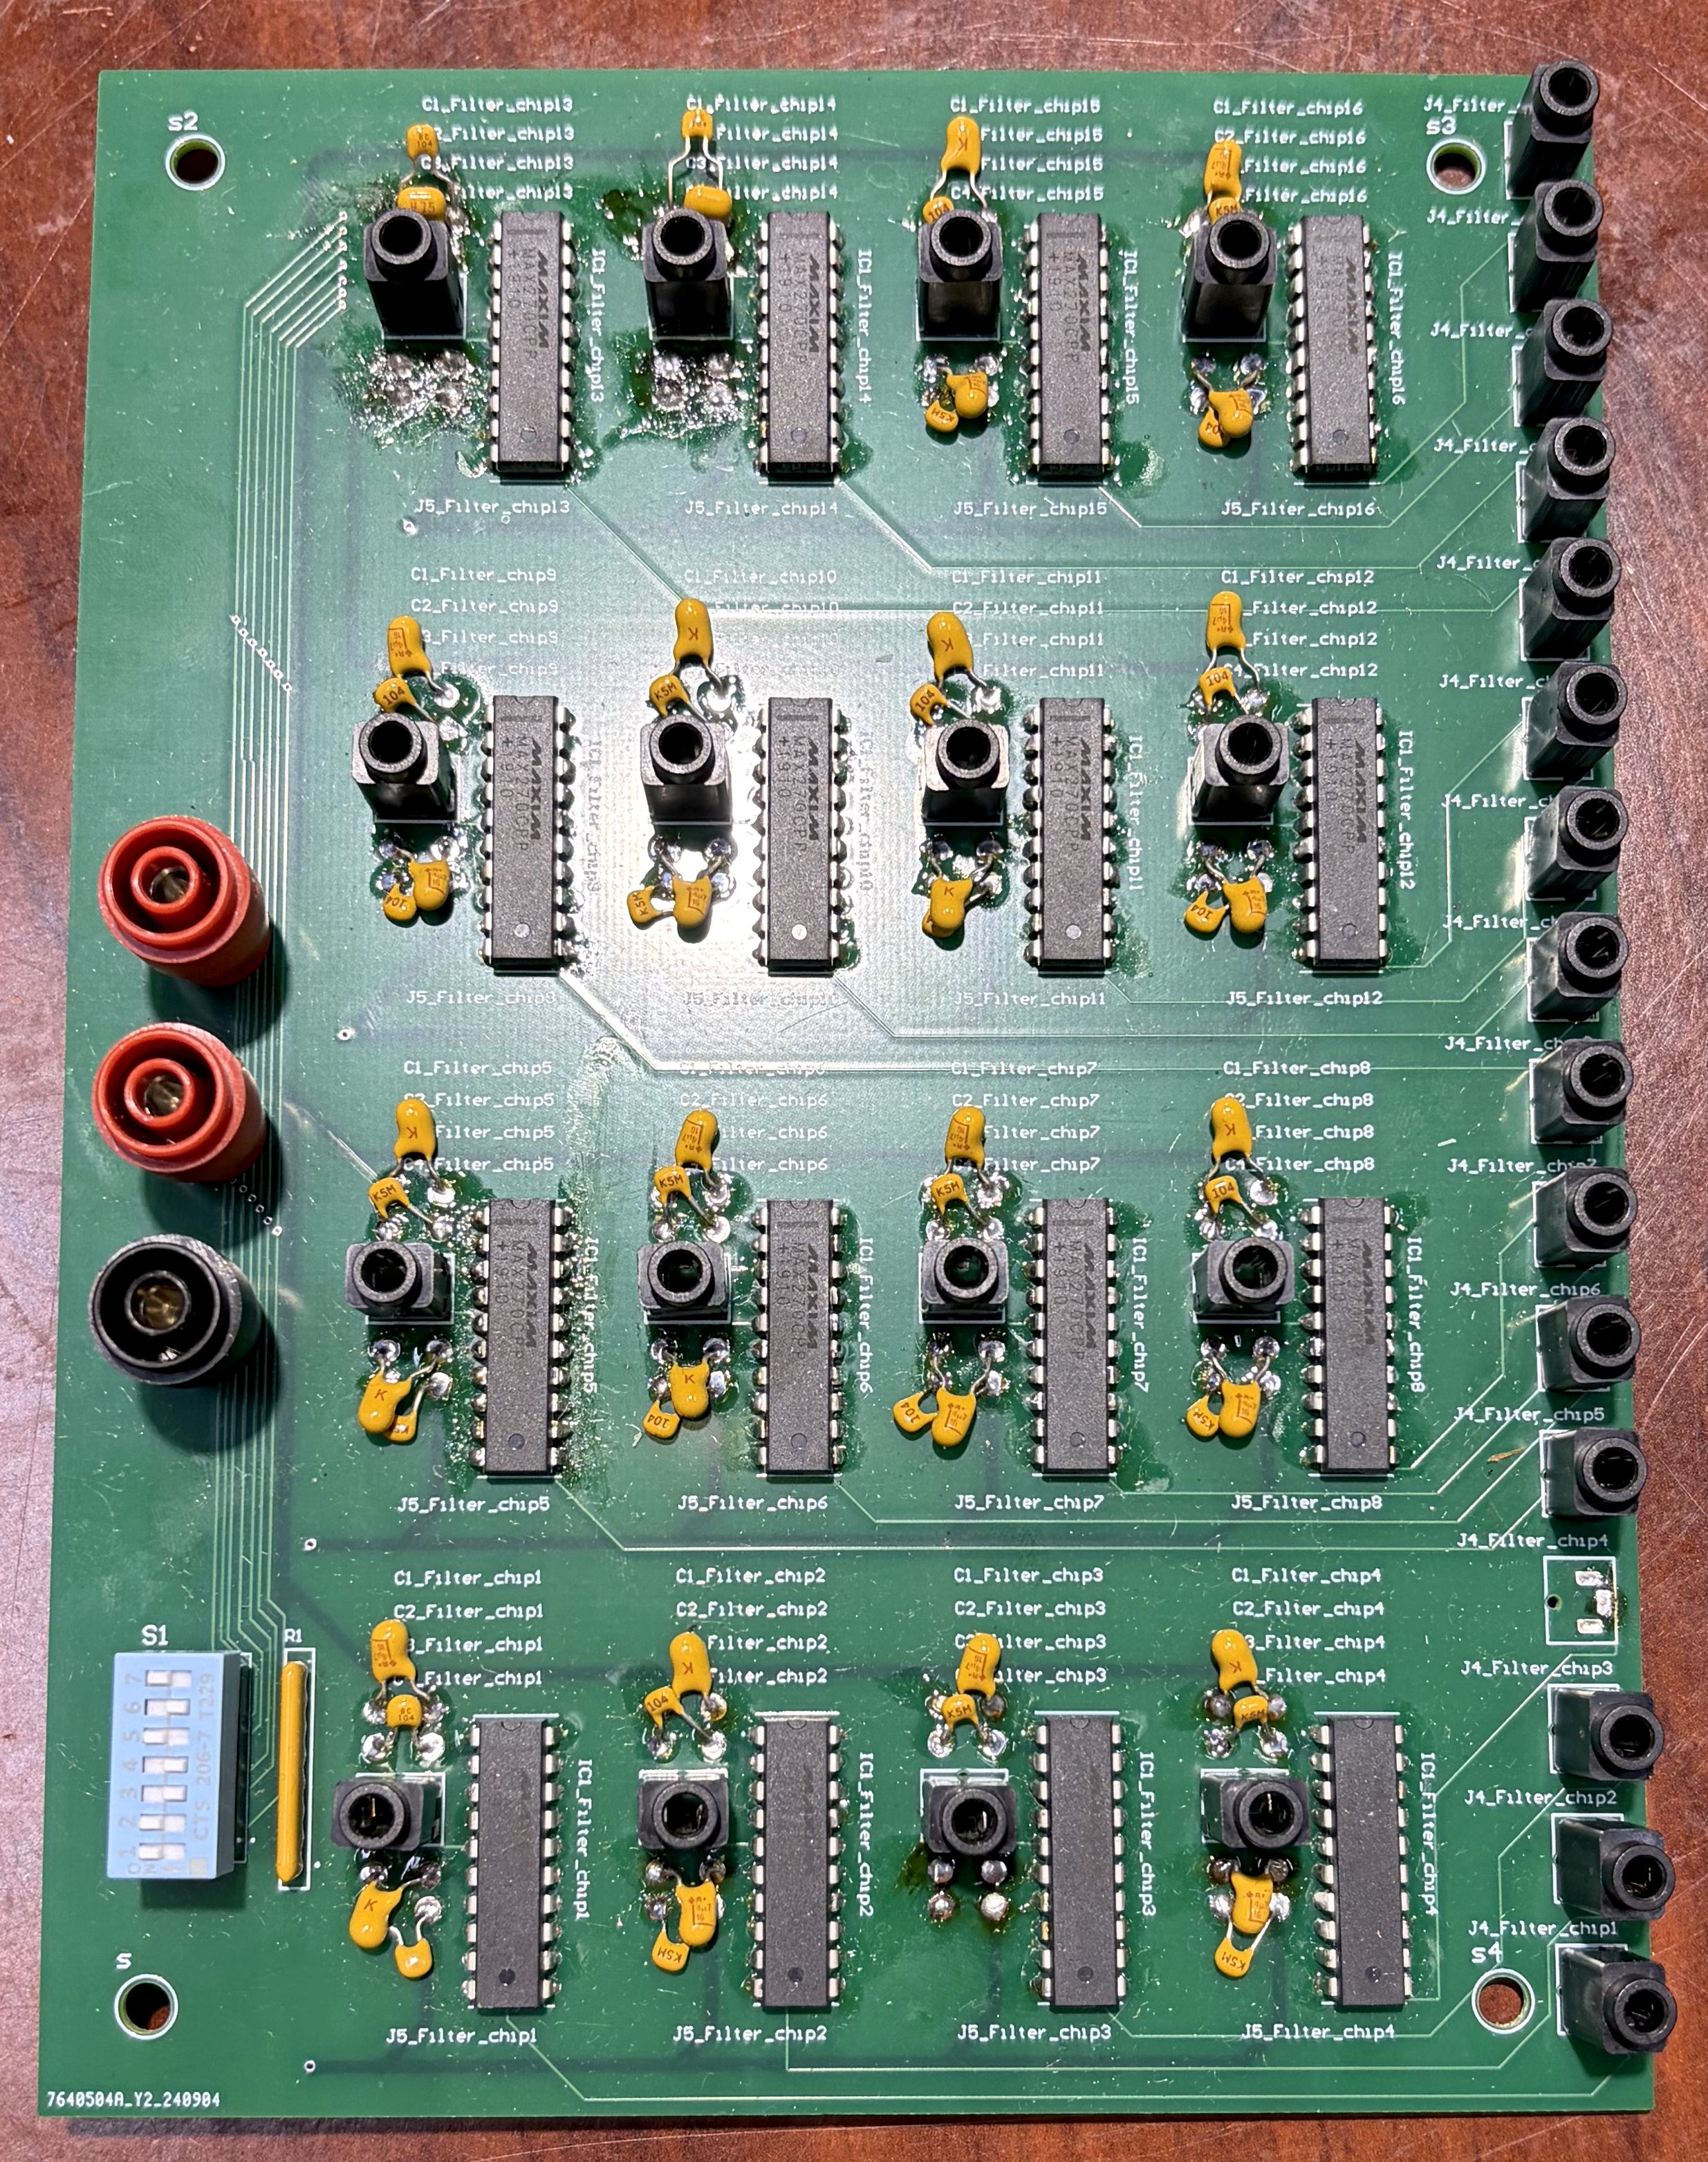
\includegraphics[width=0.48\textwidth]{Data/Photos/DAC_filter_bank.png}
    \caption{Custom DAC and filter-bank printed circuit board used for analog filtering.}
    \label{fig:filter_pcb}
\end{figure}

Each programmable filter integrated circuit contains two second-order low-pass filter sections. To achieve a steeper roll-off and improved attenuation of unwanted high-frequency components, two second-order sections were cascaded to form a fourth-order low-pass filter. Experimental testing demonstrated that the cascaded configuration provided substantially better suppression of the DAC-induced high-frequency artifacts than a single second-order filter.

\section{Adaptive filtering}

Active Noise Control (ANC) seeks to reduce unwanted sound by generating an acoustic signal that destructively interferes with the original noise. Since sound propagates as a pressure wave, a second wave of equal amplitude and opposite phase can be produced to reduce the sound pressure level at a desired location. Unlike passive noise control techniques, which rely on absorbing or blocking sound, ANC actively estimates the appropriate cancellation signal based on the measured acoustic environment.

In a feedforward ANC system, a reference microphone measures the incoming noise before it reaches the location where cancellation is desired. As the sound propagates through the environment, reflections, diffraction, and other acoustic effects alter the waveform before it reaches the error microphone. Because these environmental effects are generally unknown and may change over time, an adaptive filter is used to continuously estimate the acoustic path and generate the appropriate cancellation signal.

\begin{figure}[H]
\centering
\resizebox{0.8\textwidth}{!}{ \begin{tikzpicture}

  \node[
  % draw,
  inner sep=2.33pt,
  node font=\tiny,
  decorate=false
] at (0.66,3.16) {x(n)};
  \node[
    % draw,
    inner sep=2.33pt,
    node font=\tiny,
    decorate=false
  ] at (2.67,3.78) {d(n)};
  \node[
      % draw,
      inner sep=2.33pt,
      node font=\tiny,
      decorate=false
    ] at (2.55,3.15) {y(n)};
  \node[
    % draw,
    inner sep=2.33pt,
    node font=\tiny,
    decorate=false
  ] (node1) at (1.83,3) {h(n)};
  \draw[arrows=-Latex] (0.47,3) -- (1.37,3);
  \draw (1.37,2.81) rectangle (2.28,3.19);
  \node[
      % draw,
      inner sep=2.33pt,
      node font=\tiny,
      decorate=false
    ] at (1.82,3.62) {P(n)};
  \draw[arrows=-Latex] (0.95,3.64) -- (1.37,3.64);
  \draw (1.37,3.43) rectangle (2.28,3.81);
  \draw (0.95,3.64) -- (0.95,3.02);
  \draw (3.1,3.64) -- (2.28,3.64);
  \draw (3.1,3) circle (0.16cm);
  \draw (3.1,3.06) -- (3.1,2.94);
  \draw (3.04,3) -- (3.16,3);
  \draw[arrows=-Latex] (3.1,3.65) -- (3.1,3.16);
  \draw[arrows=-Latex] (2.28,3) -- (2.94,3);
  \draw (3.1,2.84) -- (3.1,2.6);
  \draw (3.1,2.6) -- (2.2,2.6);
  \draw (2.2,2.6) -- (2,2.81);
  \draw[arrows=-Latex] (1.64,3.19) -- (1.44,3.4);

\end{tikzpicture}
 }
\caption{Block diagram of the adaptive filtering process used for active noise cancellation.}
\label{fig:adaptive_diagram}
\end{figure}

Figure~\ref{fig:adaptive_diagram} illustrates the standard adaptive filtering model. The reference signal, $x[n]$, represents the measured disturbance before it propagates through the acoustic environment. The desired signal, $d[n]$, represents the disturbance measured at the error microphone after propagation through the unknown acoustic path. The adaptive filter, represented by the coefficient vector $\mathbf{h}$, operates on the reference signal to produce the cancellation signal.

For an adaptive filter with $M$ coefficients, the reference signal is represented as an input vector containing the current and previous reference samples,

\begin{equation}
\mathbf{x} =
\begin{bmatrix}
x[n] & x[n-1] & \cdots & x[n-M+1]
\end{bmatrix}^{T},
\end{equation}

and the adaptive filter coefficients are represented by the coefficient vector

\begin{equation}
\mathbf{h} =
\begin{bmatrix}
h_0[n] & h_1[n] & \cdots & h_{M-1}[n]
\end{bmatrix}^{T}.
\end{equation}

The filter output is calculated as the inner product of the input and coefficient vectors,

\begin{equation}
y[n] = \mathbf{x}^{T}\mathbf{h}.
\end{equation}

The objective of the adaptive filter is to continually adjust the filter coefficients so that the output $y[n]$ approaches the desired signal $d[n]$. The resulting error is therefore defined as

\begin{equation}
e[n] = d[n] - y[n].
\end{equation}

The adaptive algorithm attempts to minimize the mean squared error between the desired signal and the filter output. The corresponding cost function is

\begin{equation}
J[n] = E\left[e^2[n]\right]
= E\left[\left(d[n]-\mathbf{x}^{T}\mathbf{h}\right)^2\right].
\end{equation}

Expanding the squared term gives

\begin{equation}
J[n] = E\left[d^2[n]-2d[n]\mathbf{x}^{T}\mathbf{h}
+\left(\mathbf{x}^{T}\mathbf{h}\right)^2\right].
\end{equation}

To determine the filter coefficients that minimize the cost function, the gradient of $J[n]$ with respect to the filter coefficient vector is computed as

\begin{equation}
\nabla_{\mathbf{h}} J
=
-2E\left[\mathbf{x}d[n]\right]
+
2E\left[\mathbf{x}\mathbf{x}^{T}\right]\mathbf{h}.
\end{equation}

The optimal solution requires knowledge of the statistical expectations of the input signal, which are generally unavailable during real-time operation. The Least Mean Squares (LMS) algorithm addresses this problem by replacing the expected gradient with its instantaneous estimate,

\begin{equation}
\nabla_{\mathbf{h}} J
\approx
-2e[n]\mathbf{x}.
\end{equation}

Although this approximation does not produce the exact gradient at every iteration, the average behavior of the algorithm follows the direction of steepest descent. This allows the filter coefficients to converge toward the minimum of the mean squared error surface through an iterative steepest-descent process.

Using this instantaneous gradient, the filter coefficients are updated according to

\begin{equation}
\mathbf{h}[n+1]
=
\mathbf{h}[n]
+
\mu e[n]\mathbf{x}[n],
\end{equation}

where $\mu$ is the adaptation step size. The value of $\mu$ determines the convergence characteristics of the algorithm. Larger values of $\mu$ increase the adaptation rate but may lead to instability or increased steady-state error, while smaller values improve stability at the expense of slower convergence. Consequently, the step size must be selected to balance convergence speed and stability for the desired application.

Initially, the LMS algorithm was used during testing due to its computational efficiency and simplicity while the real-time computational constraints of the system were still being determined. The reduced computational complexity of LMS allowed early testing of acoustic noise cancellation performance and evaluation of the overall system architecture.

Although LMS is computationally efficient, its convergence rate depends on the eigenvalue spread of the input correlation matrix. In highly correlated signals, such as speech and snoring, LMS may require many iterations before converging. Since active noise control systems must adapt quickly to changing acoustic environments, a faster adaptive algorithm is desirable.

Unlike LMS, Recursive Least Squares (RLS) minimizes an exponentially weighted least-squares cost function rather than relying on a stochastic gradient approximation. Consequently, RLS typically converges significantly faster than LMS but requires substantially more computation because a matrix inverse, or an equivalent recursive update, must be maintained.

The Fast Array Recursive Least Squares (FARLS) algorithm exploits the recursive structure of the RLS solution to reduce the computational complexity associated with conventional matrix operations. Rather than explicitly computing the full inverse correlation matrix at each iteration, FARLS recursively updates intermediate quantities, resulting in convergence characteristics similar to RLS while reducing the computational cost.

In the FARLS formulation used in this work, the input vector is denoted by $\mathbf{u}[n]$ and the adaptive filter coefficient vector is denoted by $\mathbf{w}[n]$. The input vector contains the current and previous samples used by the adaptive filter and can be represented as

\begin{equation}
\mathbf{u} =
\begin{bmatrix}
x[n] & x[n-1] & \cdots & x[n-M+1]
\end{bmatrix}^{T}.
\end{equation}

The FARLS filter output is therefore calculated from the input and coefficient vectors as

\begin{equation}
y[n] = \mathbf{w}^{T}\mathbf{u}.
\end{equation}

The FARLS algorithm recursively updates the coefficient vector as new samples are received. The general procedure used in this work is summarized in Algorithm~\ref{alg:farls}.

\begin{algorithm}[H]
\caption{FARLS Adaptive Filtering Procedure}
\label{alg:farls}
\begin{algorithmic}

\Require Input sample $x(n)$, desired signal $d(n)$
\Require Filter length $M$, forgetting factor $\lambda$

\State Initialize filter coefficients $\mathbf{w}[0]$ and FARLS recursive array $A$

\For{$n=1,2,\ldots,N$}

\State Update the input vector $\mathbf{u}$ and recursive quantities in $A$

\State Calculate and apply the circular rotation parameters

\State Calculate and apply the hyperbolic rotation parameters

\State Update the recursive quantities using $\lambda$

\State Calculate the filter output:
\[
y[n] = \mathbf{w}^{T}\mathbf{u}
\]

\State Calculate the prediction error:
\[
e[n] = d[n]-y[n]
\]

\State Update the filter coefficients:
\[
w_j[n] = w_j[n-1] + g_j[n]e[n],
\qquad j=1,\ldots,M
\]

\EndFor

\State \Return $\mathbf{w}[n]$

\end{algorithmic}
\end{algorithm}

The FARLS procedure begins by initializing the filter coefficients and the recursive array used to store the intermediate quantities required by the algorithm. At each iteration, a new input sample is incorporated into the input vector, which contains the current and previous samples used by the adaptive filter. The recursive quantities in the array are then updated using the new input information and the state retained from the previous iteration.

The recursive update is performed using circular and hyperbolic rotations. These rotations transform the intermediate quantities in the FARLS array while avoiding the explicit formation and inversion of the input correlation matrix required by conventional RLS. The forgetting factor is also incorporated during these recursive updates, allowing older samples to have progressively less influence on the least-squares solution. This enables the algorithm to continuously adapt as new samples are received.

After the recursive quantities have been updated, the current filter output is calculated from the input vector and filter coefficients, and the prediction error is determined as the difference between the desired signal and the filter output. The prediction error and the calculated gain are then used to update the filter coefficients. This coefficient update allows the filter to respond to the most recent error while retaining information from previous iterations through the recursive state variables. This process is repeated for each incoming sample, allowing the FARLS filter to continuously adapt to changes in the input signal.

\section{Experimental Setup}

The experimental platform consisted of a workstation running the Ubuntu Linux operating system. All signal processing and adaptive filtering algorithms were implemented in the C programming language and compiled using the GNU Compiler Collection (GCC). The workstation was equipped with an Intel processor, an NVIDIA graphics processing unit (GPU), and sufficient system memory to satisfy the real-time computational requirements of the active noise control algorithms.

Audio acquisition and playback were performed using the PCIe66-16AI32SSC analog-to-digital converter (ADC) and the 66-16AO16 digital-to-analog converter (DAC), respectively. The system operated at a sampling frequency of 8~kHz with a 16-bit sample resolution. The adaptive filtering algorithms processed the acquired audio in real time, continuously generating the cancellation signals transmitted to the loudspeaker array.

\begin{figure}[H]
    \centering
    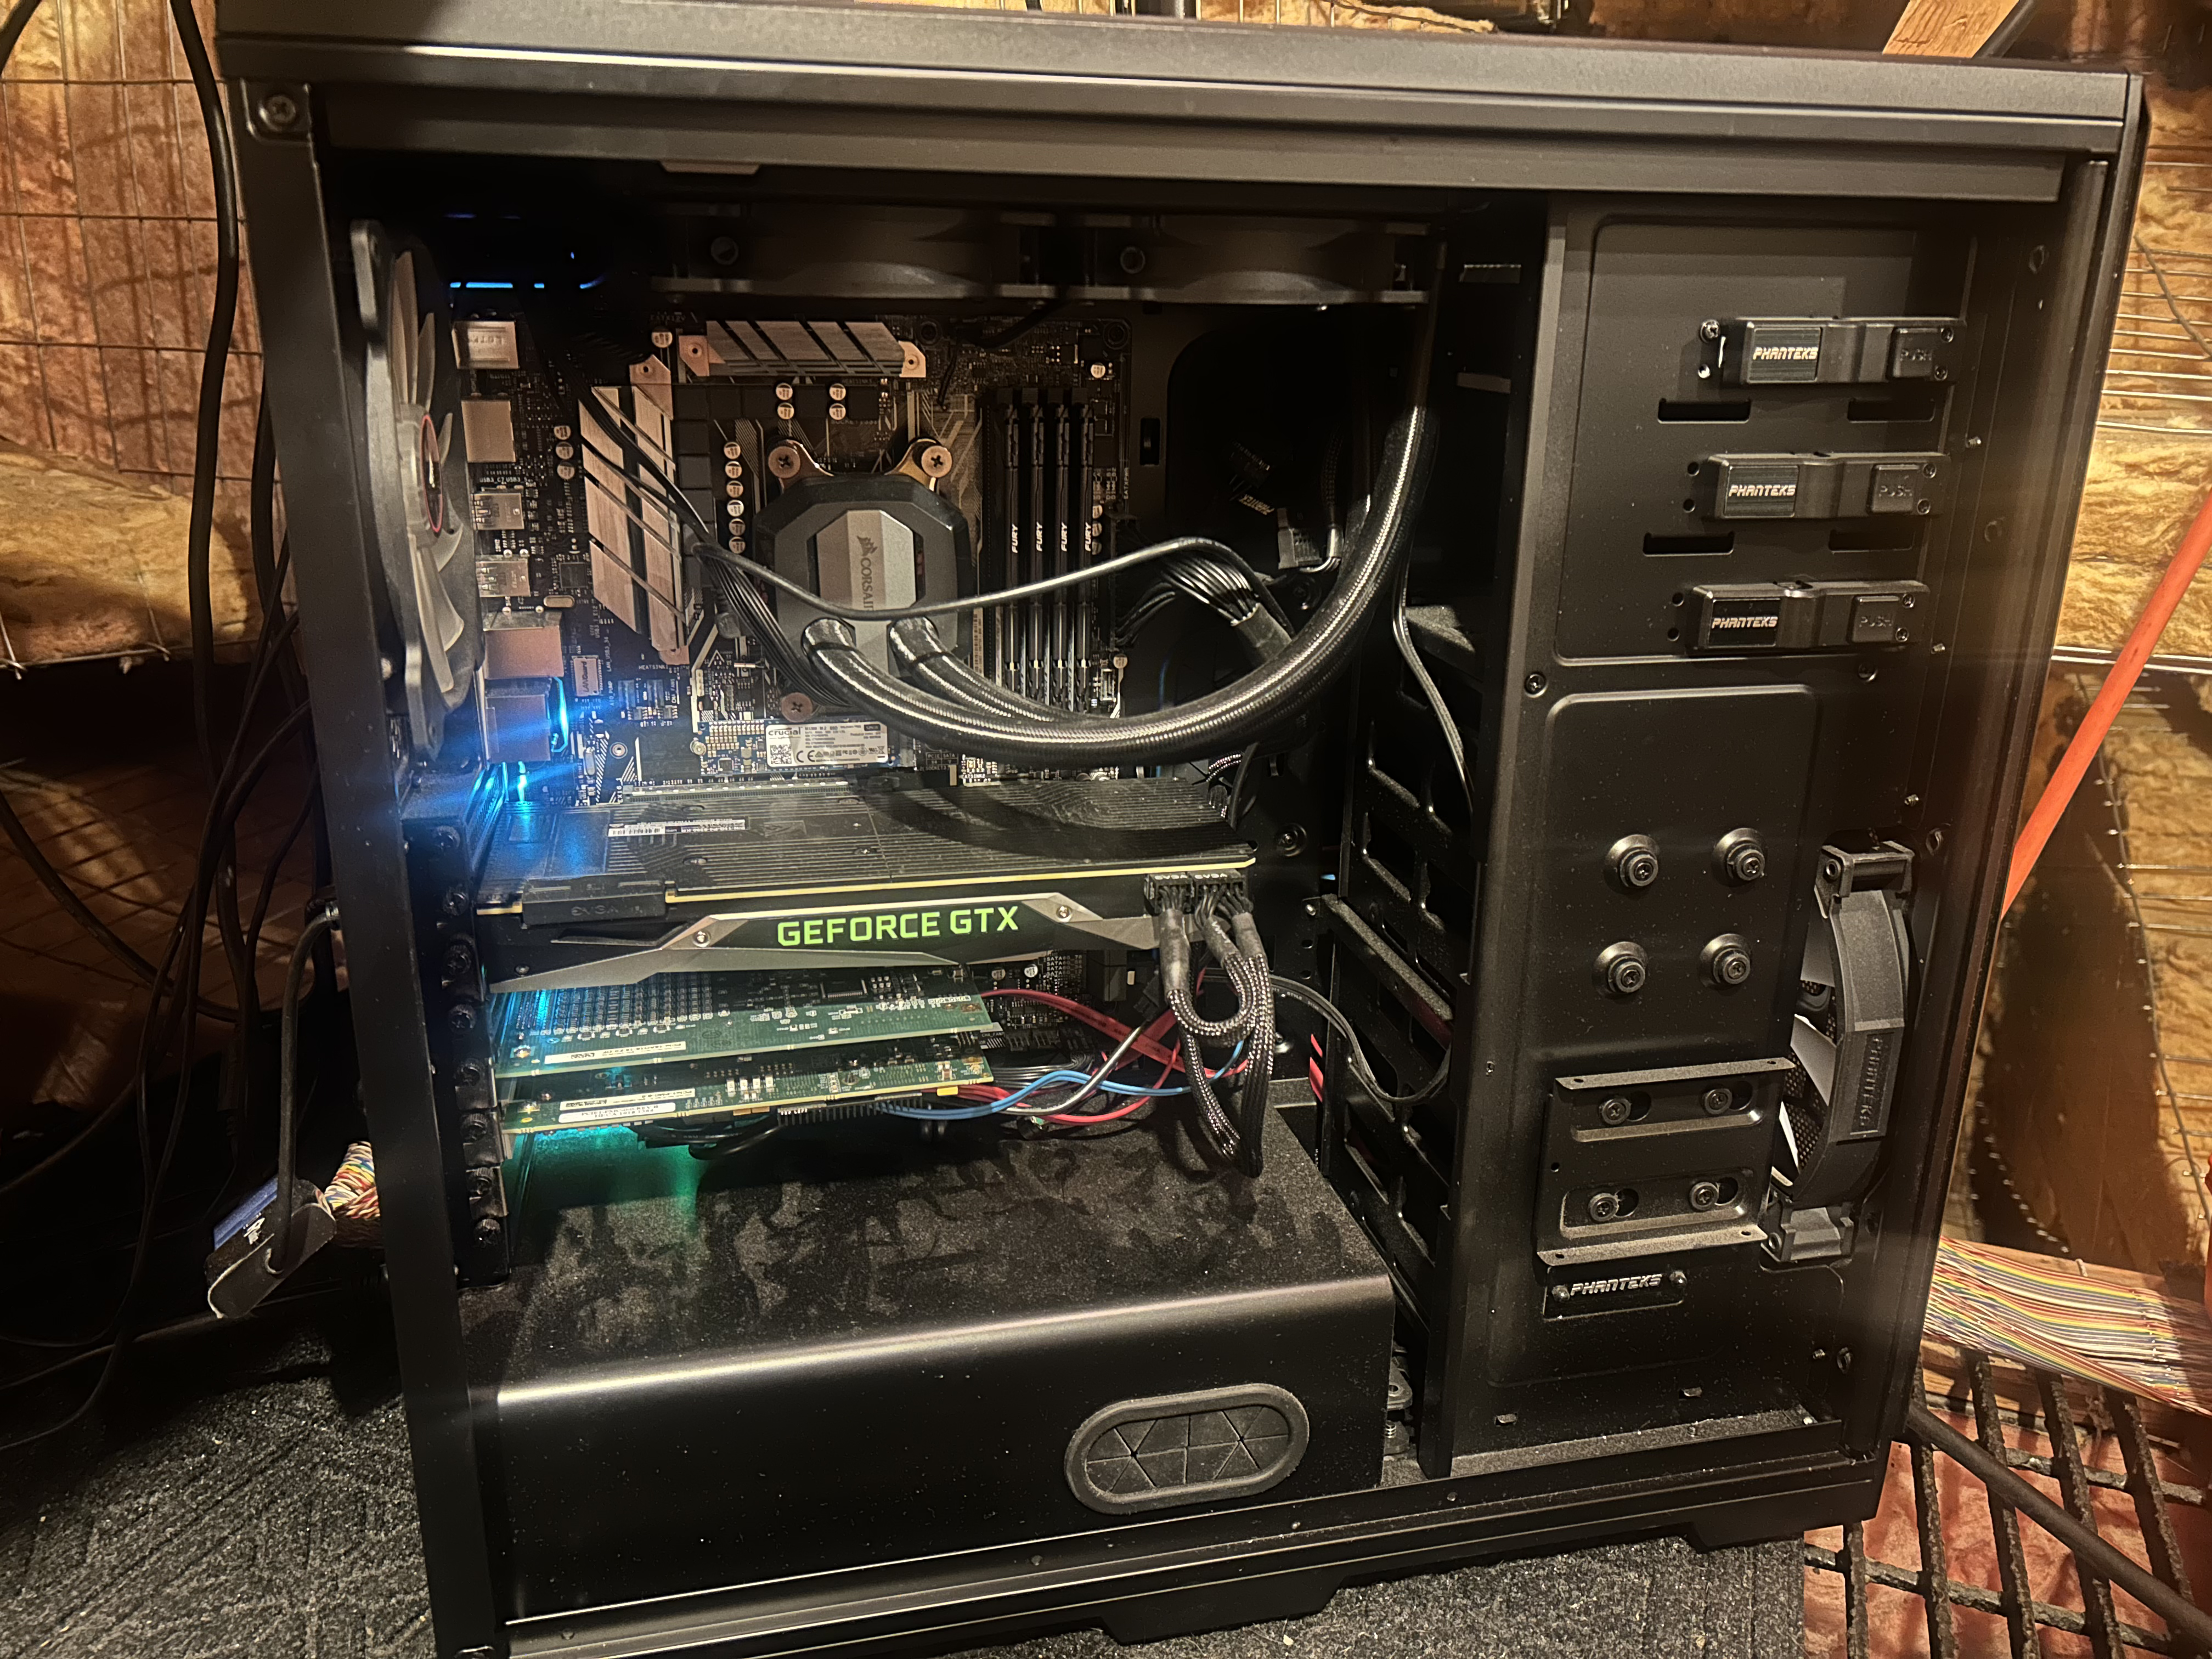
\includegraphics[width=0.8\textwidth]{Linux_computer.png}
    \caption{Linux-based workstation used for real-time signal processing and adaptive noise cancellation.}
    \label{fig:linux_setup}
\end{figure}

\begin{figure}[H]
  \centering
    \resizebox{0.8\textwidth}{!}{ \begin{tikzpicture}
  \draw (1.19,4.44) circle (0.58cm);
  \node[
    node font=\tiny,
    align=center,
    text width=1.1cm
  ] (node5) at (1.19,4.44) {Snore\\Source};
  
  \node[
    node font=\tiny,
    align=center,
    text width=1.5cm
  ] at (2.01,1.81) {Adaptive\\Algorithm};
  
  \node[node font=\tiny] at (0.89,1.91) {$x(n)$};
  \node[node font=\tiny] at (6.43,2.07) {$H1$};
  \node[node font=\tiny] at (6.43,1.51) {$HN$};
  \draw (0.33,1.79) circle (0.21cm);
  \draw (5.47,2.07) circle (0.1cm);
  \node[draw, shape=trapezium, rotate=90] (node2) at (5.7,2.07) {};
  \draw (5.47,1.51) circle (0.1cm);
  \node[draw, shape=trapezium, rotate=90] (node3) at (5.7,1.51) {};

  \draw (0.06,2) -- (0.6,2);
  \draw[arrows=-Latex] (0.33,3.07) -- (0.33,2);
  \draw[arrows=-Latex] (0.54,1.79) -- (1.2,1.79);
  \draw (1.19,1.44) rectangle (2.83,2.17);
  \draw (2.02,3.02) circle (0.25cm);

  \draw (2.12,3.16) -- (1.93,3.16) -- (2.08,3.02) -- (1.94,2.91) -- (2.12,2.91);
  \draw[arrows=-Latex] (2.01,2.77) -- (2.01,2.17);
  \draw[arrows=-Latex] (2.83,1.81) -- (3.32,1.81);
  \draw (3.29,1.43) rectangle (4.67,2.17);

  \node[
    node font=\tiny,
    align=center,
    text width=1.3cm
  ] at (3.97,1.8) {Array\\Algorithm};
  
  \draw (3.32,2.63) rectangle (4.7,3.37);
  \node[
    node font=\tiny,
    align=center,
    text width=1.3cm
  ] (node4) at (4,3) {Array\\Algorithm};
  
  \draw[arrows=-Latex] (4.67,2.07) -- (5.39,2.07);
  \draw[arrows=-Latex] (4.67,1.52) -- (5.39,1.52);
  \draw[fill=black] (5.27,1.93) circle (0.04cm);
  \draw[fill=black] (5.27,1.8) circle (0.04cm);
  \draw[fill=black] (5.27,1.67) circle (0.04cm);
  \draw[fill=black] (5.28,3.11) circle (0.04cm);
  \draw[fill=black] (5.28,2.98) circle (0.04cm);
  \draw[fill=black] (5.28,2.85) circle (0.04cm);
  \draw[fill=black] (6.38,1.86) circle (0.04cm);
  \draw[fill=black] (6.38,1.73) circle (0.04cm);
  \draw (0.33,3.06) -- (0.9,3.93);
  \draw (6.1,1.95) rectangle (6.71,2.19);
  \draw (6.1,1.39) rectangle (6.71,1.63);
  \node[node font=\tiny] at (6.44,3.25) {$H1$};
  \node[node font=\tiny] at (6.44,2.69) {$HN$};
  \draw[fill=black] (6.39,3.04) circle (0.04cm);
  \draw[fill=black] (6.39,2.91) circle (0.04cm);
  \draw (6.11,3.13) rectangle (6.72,3.37);
  \node[node font=\tiny] at (4.23,4.44) {$HP$};
  \draw (3.89,4.32) rectangle (4.5,4.56);
  \draw (6.11,2.57) rectangle (6.72,2.81);
  \draw (6.71,2.07) -- (6.9,2.07);
  \draw (6.71,1.5) -- (7.1,1.5);

  \draw (7.58,4.44) circle (0.58cm);
  \node[node font=\tiny] at (7.58,4.44) {Hearer};
  \draw[arrows=-Latex] (node2.south) -- (6.11,2.07);
  \draw[arrows=-Latex] (node3.south) -- (6.11,1.51);
  \draw[arrows=-Latex] (6.9,2.07) -- (7.4,3.91);
  \draw[arrows=-Latex] (7.1,1.5) -- (7.54,3.86);
  \draw[arrows=-Latex] (6.92,3.27) -- (6.7,3.27);
  \draw[arrows=-Latex] (6.92,2.69) -- (6.7,2.69);
  \draw (6.92,2.69) -- (7.27,3.94);
  \draw (6.92,3.27) -- (7.2,4);

  \draw[rotate=-90] (-3.25,5.71) circle (0.21cm);
  \draw[rotate=-90] (-2.69,5.71) circle (0.21cm);
  \draw[rotate=-90] (-2.87,5.92) -- (-2.48,5.92);
  \draw[rotate=-90] (-3.46,5.92) -- (-3.07,5.92);
  \draw[arrows=-Latex] (6.11,3.25) -- (5.9,3.25);
  \draw[arrows=-Latex] (6.11,2.69) -- (5.9,2.69);
  \draw[arrows=-Latex] (5.5,2.69) -- (4.69,2.69);
  \draw[arrows=-Latex] (5.5,3.25) -- (4.69,3.25);
  \draw[arrows=-Latex] (3.32,3) -- (2.26,3);

  \draw[arrows=-Latex] (1.76,4.44) -- (3.89,4.44);
  \draw[arrows=-Latex] (4.49,4.44) -- (7,4.44);
  
  \node[node font=\tiny] at (2.75,4.59) {s(n)};
  \node[node font=\tiny] at (2.8,3.14) {e(n)};
  \node[node font=\tiny] at (3.06,2) {y(n)};
  \node[node font=\tiny] at (5.25,4.6) {r(n)};
\end{tikzpicture}
 }
    \caption{Block diagram illustrating the signal flow through the active noise cancellation system.}
    \label{fig:sys_block_diagram}
\end{figure}

Figure ~\ref{fig:sys_block_diagram} illustrates the overall signal flow of the experimental platform. Audio signals acquired by the microphone array were digitized by the ADC and transferred to the Linux workstation for real-time processing. After the adaptive filtering algorithm computed the cancellation signal, the processed audio was transmitted through the DAC, passed through the analog low-pass filter bank described in the previous section, and reproduced by the loudspeaker array.

The ADC and DAC cards interfaced with the experimental hardware through ribbon cable connections. Each ribbon cable was connected to a custom interface enclosure that converted the ribbon cable outputs into standard 3.5~mm audio connectors. The microphone array was connected to the ADC interface enclosure, while the loudspeaker array was connected to the DAC interface enclosure through the programmable analog low-pass filter bank.

The experimental hardware consisted of a 16-element microphone array and a 16-element loudspeaker array mounted on the adjustable support structure described in Section~3.2. The microphone spacing was adjustable, with experiments performed using a spacing of approximately 0.08575 meters. The speaker array was similarly adjustable, allowing different acoustic geometries to be evaluated while maintaining repeatable positioning throughout the experiments.

All experiments were conducted inside an anechoic chamber to minimize reflections and external acoustic interference. This environment allowed the performance of the microphone array, beamforming algorithms, and adaptive noise control system to be evaluated under controlled acoustic conditions.

To evaluate system performance, known audio signals were used as the disturbance source. Test signals were generated using an external loudspeaker positioned at predetermined locations relative to the microphone array. These controlled acoustic sources provided repeatable input signals for evaluating the fractional delay interpolation, beamforming, and adaptive filtering algorithms. Experimental results obtained using this setup are presented and discussed in Chapter~4.

% Local Variables:
% TeX-master: "newhead"
% End:
